\documentclass[a4paper]{report}
 \usepackage[14pt]{extsizes}
 \usepackage[utf8]{inputenc}
 \usepackage[T1]{fontenc}
 \usepackage[french]{babel}
 \usepackage{makeidx}
 \usepackage{graphicx} 
 \title{RAPPORT DU PROJET STL \\ TIKZ}
 \author{ANCELIN Maxime & DIAKHATE Aminata}

 \maketable    %pour générer l'index

\begin{document}          %début du document

 \maketitle
 \tableofcontents
 \newpage


 \newpage
 \section{Introduction}
  Dans le cadre de notre enseignement universitaire à l'UPMC(Université Pierre Marie Curie) en master Informatique, nous devons réaliser un projet. 
  
  \section{Présentation du projet}
  \subsection{Etat Actuel}
  LaTex(Lamport TEX) est un langage et un système de composition de documents. Du fait de sa relative simplicité, il est souvent utilisé dans les domaines techniques et scientifiques pour la production d'un contenu complexe (équations, graphes, ...) ayant une mise en forme standard. Afin d'inclure ces contenus complexes dans les documents en restant dans l'environnement LaTex, LaTex dispose d'un package TikZ permettant d'inclure des figures au format PDF. En effet, TikZ permet d'obtenir des figures géométriques complexes précise et d'une grande qualité. Cependant son apprentissage n'est pas évident. 
  \subsection{Motivation}
  Notre encadrant, qui est lui-même un utilisateur de TikZ, a souhaité faciliter son utilisation afin de permettre à un plus grand nombre d'utilisateurs de profiter des avantages de TikZ sans passer par son apprentissage. Pour ce faire, il nous propose donc de mettre en place une interface graphique permettant la construction  visuelle (et non textuelle) des figures.
  \newline
  Pour ce projet que nous devions réaliser dans le cadre de notre master, nous avions souhaité, avant même de 
connaître les projets proposés, de choisir un projet qui nous permettrait de nous rapprocher le plus des projets qu'on pourrait rencontrer dans le monde professionnel et qui 
  \subsection{Objectifs}
Notre objectif est de pouvoir présenter au terme de ce projet une interface graphique qui permettrait à l'utilisateur de pouvoir créer des graphes non plus textuellement mais visuellement. L'interface graphique devra aussi permettre à l'utilisateur de rédiger du code TikZ et visionner le graphe correspondant ou encore modifier le graphe en bougeant les noeuds sélectionnés ou en modifiant leurs propriétés grâce à un menu.
Toute modification apportée au graphe devra mettre à jour le code source correspondant et vice-versa. 
  \section {Gestion du projet}
  \subsection{Choix technologiques}
  Pour la réalisation de notre projet, notre encadrant nous a recommandé l'utilisation d'un langage de script tel que Python ou Ruby, permettant l'interfaçage avec des outils externes (notamment pdflatex avec le paquet "preview") et les manipulations textuelles simples (expressions rationnelles etc.), et proposant de plus des bibliothèques portables pour les interfaces utilisateurs (Gtk, Qt, WxWindows, etc.). Même si notre encadrant nous a vivement conseillé l'utilisation de Python nous avons quand même choisi de faire notre projet avec Perl. 

Perl nous a semblé être un bon choix de langage car il est adapté au traitement et manipulation de fichiers texte du fait de l'intégration des expressions régulières dans la syntaxe même du langage or nous voulions manipuler des fichers LaTex et Tikz; de plus perl est portable sur la plupart des systèmes d'exploitation, il devient même populaire sous Windows grâce à la distribution gratuite ActivePerl. 
Pour l'interface utilisateur nous avons choisi la bibliothèque Qt comme nous le conseillait notre encadrant. Au final nous avons donc utiliser PerlQt qui allie la souplesse, la puissance et le design élégant de Qt au langage Perl. Pour l'installater, nous avons dû choisir entre deux versions de PerlQt4:
\begin{itemize}
 \item Une version avec une vue sur Qt-sys.org publié par l'utilisateur "vadiml" et qui n'a pas été mise à jour depuis Février 2008
 \item Une autre avec une vue sur code.google.com publié par "chrisburel@gmail" qui semblait plus complète et surtout activement maintenue puisque la dernière version datait de quelques jours seulement.
\end{itemize}
  Notre choix c'est donc naturellement porté sur la version proposée par "chrisburel@gmail".
  \newline 
  Pour notre interface graphique, nous avions besoin d'un éditeur qui nous permettrait d'écrire du code Tikz. Pour cela nous avons choisi Scintilla qui est un composant d'édition de code open source. En effet Scintilla a beaucoup de fonctionnalités qui rendent l'édition de code plus facile telles que la coloration syntaxique, la gestion des numéros de ligne dans la marge, les points d'arrêts pour le débogueur, etc.
  \newline
  Au début de notre projet nous n'avions pas utiliser de gestionnaire de version car nous travaillions le plus souvent ensemble ; mais pendant les vacances scolaires du mois d'avril où la distance ne nous permettait pas de continuer à travailler ensemble, nous avons installé git qui est un logiciel de gestion de versions décentralisé libre. 
\subsection{Difficultés} 
\subsubsection{Installation de perlqt4}

L' installation de perlqt4 nous a pris un peu plus d' une semaine,
car il nous manquait des dépendances.

Au fur et a mesure que nous découvrions ce qu' il fallait ajouter,
nous avons enrichi un script d' installation afin de rendre la reinstallation
plus facile pour les utilisateurs finaux de notre application. Ce
script a été conçu pour fonctionner sous Ubuntu 12.04 et devrait marcher
sans encombre sous Debian.

Sous ces linux, il suffit de lancer \textbf{script\_intall\_all.sh}
afin d' installer perlqt4, Scintilla et tout les packages et modules
perl requis au fonctionnement de l' application.

\subsubsection{Identification des objets Tikz}

Afin d' identifier indépendament chaque objet Tikz, nous attribuons à chaque n{\oe}ud une couleur unique.

L' idée de base est de générer une image de la même taille que l'
image originale où chaque objet Tikz aurait une couleur différente. 
\subsection{Architecture}
  DIAGRAMME DES CLASSES EN MOINS DETAILLE   
\subsection{Gestion du temps}
  DIAGRAMME REPRESENTANT LE TPS PASSE POUR: APPRENDRE TIKZ ET LATEX, INSTALLER LES LOGICIELS, CREER L'INTERFACE GRAPHIQUE BASIQUE, ECRIRE LE PARSER, IDENTIFIER ET DEPLACER UN OBJET, AFFICHER ET MODIFIER LES PROPRIETES DE L'OBJET SELECTIONNE, REDIGER LE RAPPORT, REDIGER LA PRESENTATION, PARSER LES MESSAGES D'ERREUR.
\subsection{Résultats}
  Nous allons à présent vous présenter en images les résultats de notre projet .
\newline
  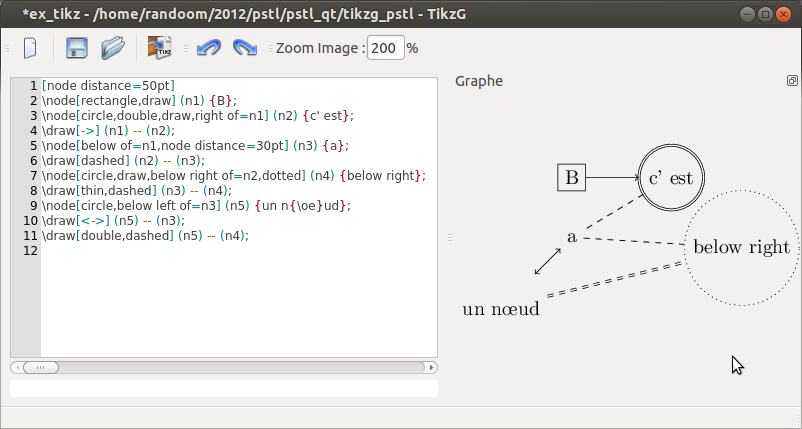
\includegraphics[width=15cm, height=10cm]{img/r_1.png} 
\newline
figure 1: génération du graphe à partir du code tikz édité
\\
\\
\\
\\
  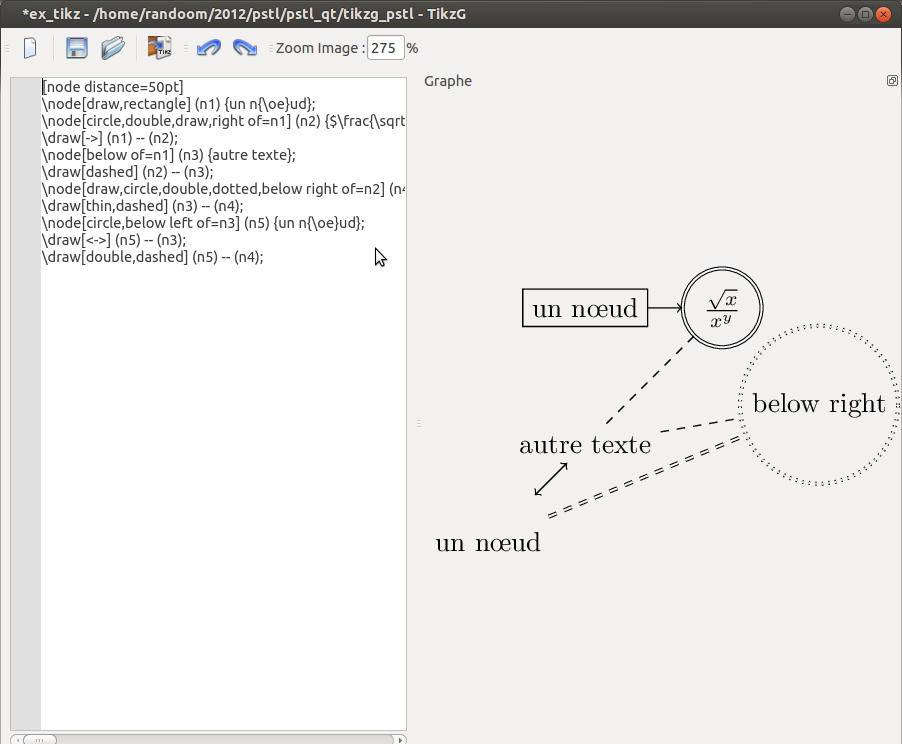
\includegraphics[width=15cm, height=10cm]{img/r_41.png} 
\\
figure 2: zoom et désactivation de la coloration et des numéros de ligne dans la marge
\newline
\\
\\
\\
\\
  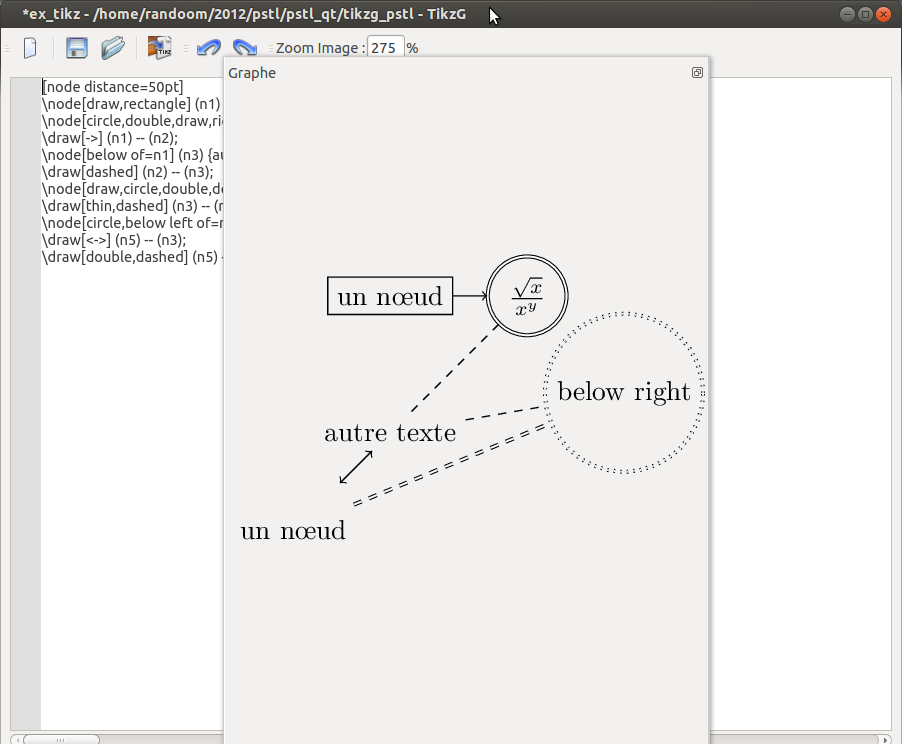
\includegraphics[width=15cm, height=10cm]{img/r_42.png} 
\\
figure 3: fenêtre du graphe flottante
\newline
\\
\\
\\
\\
  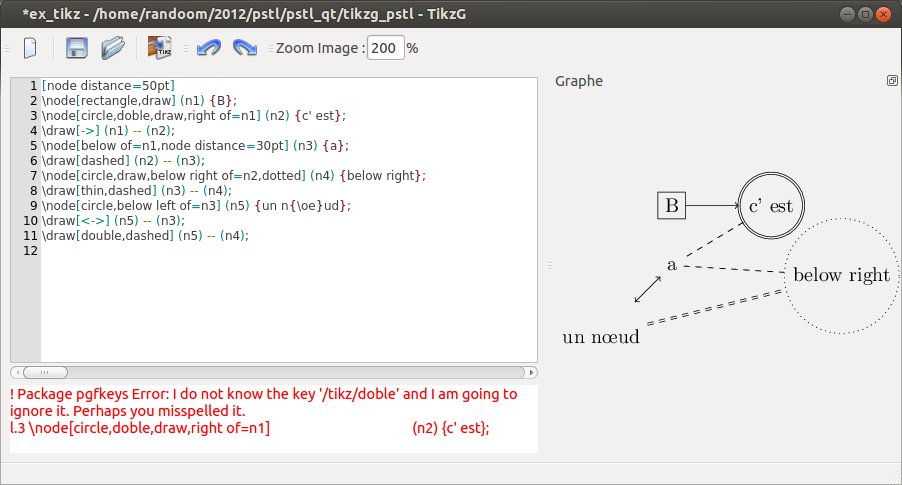
\includegraphics[width=15cm, height=10cm]{img/r_2.png} 
\\
figure 4: gestion d'erreurs
\\
\\
	Comme nous pouvons le constater sur la figure 1, le graphe est généré à partir du code Tikz écrit dans l'éditeur de texte. Cette génération est relancée automatique au bout d'une seconde d'inactivité. L'utilisateur pourra choisir de cacher les numéros de ligne ou de désactiver la coloration syntaxique en décochant les cases correspondantes dans la barre de menu ; il pourra aussi définir la valeur du zoom dans la barre d'outil ou zoomer avec la molette de la souris. En effet, sur la figure 1 on peut noter l'affichage des numéros de ligne, la coloration syntaxique du code et la valeur du zoom qui est de 200\%
alors que sur la figure 2 l'affichage des numéros de ligne est désactivée de même que la coloration syntaxique et la valeur du zoom vaut 275\% après un zoom avec la molette de la souris.

De plus, comme l'atteste les figures 3 et 4, les erreurs sont gérees et la fenêtre du graphe peut être détachée de l'interface et déplacée sans que cela ne modifie ses fonctionnalités.
\newline
  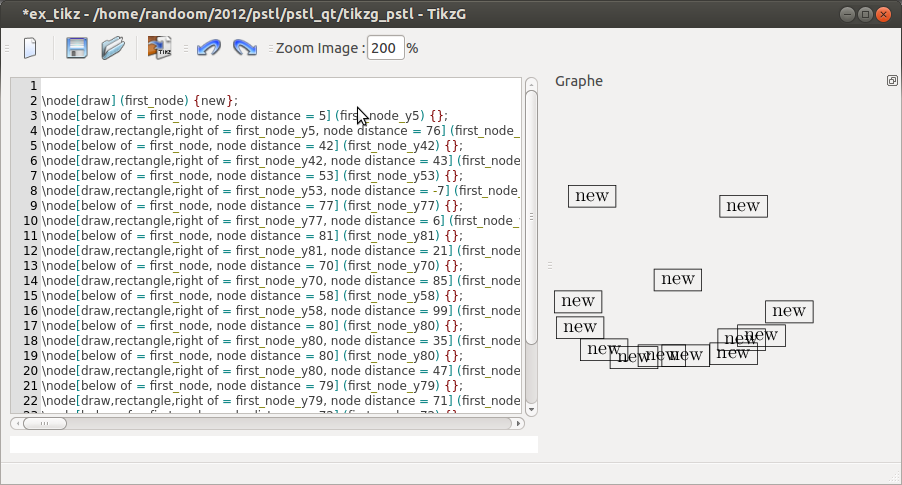
\includegraphics[width=15cm, height=10cm]{img/r_6.png} 
\\
  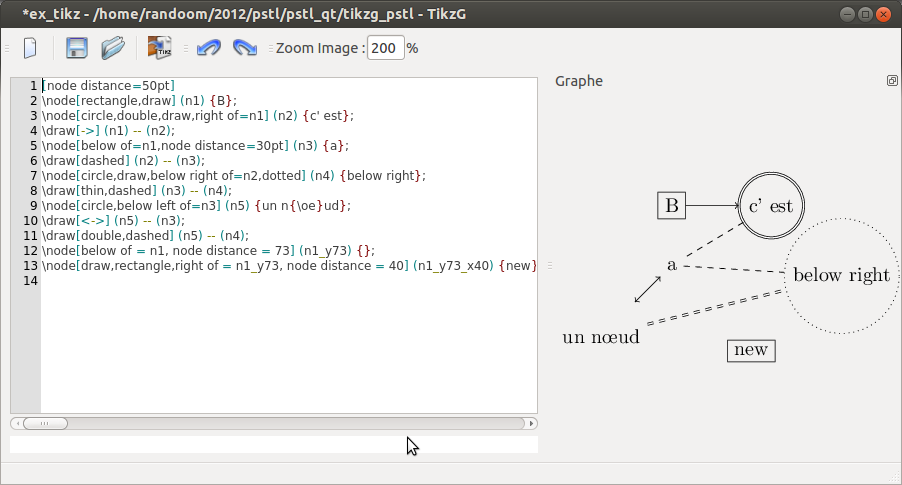
\includegraphics[width=15cm, height=10cm]{img/r_3.png}
\\ 
figures 5: création graphique d'un n{\oe}ud
\newline
  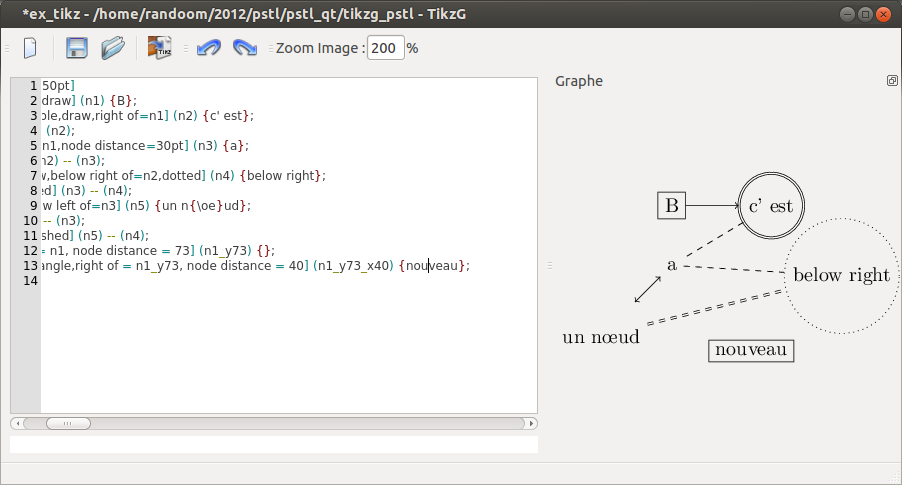
\includegraphics[width=15cm, height=10cm]{img/r_5.png} 
figure 6: modification textuelle des propriétés d'un n{\oe}ud
\\
\\
Un clic droit sur l'interface graphique permet de créer un n{\oe}ud à cet l'endroit qu'on pourra par la suite modifier textuellement ou graphiquement. Le code correspondant au noeud ainsi créé est automatique ajouter au code du graphe (figures 5 et 6). 
\newline
  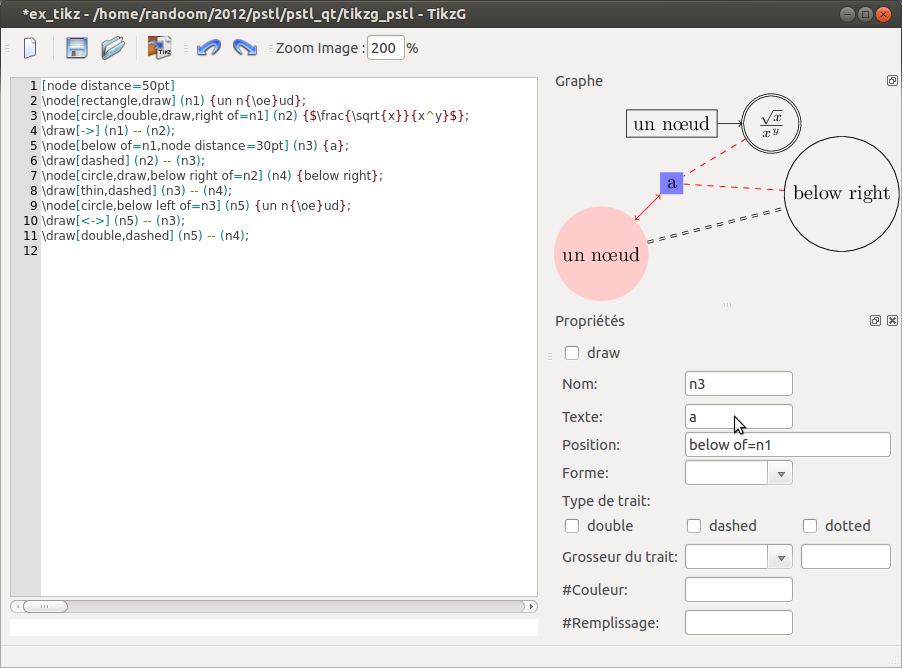
\includegraphics[width=15cm, height=10cm]{img/r_8.png} 
\\
  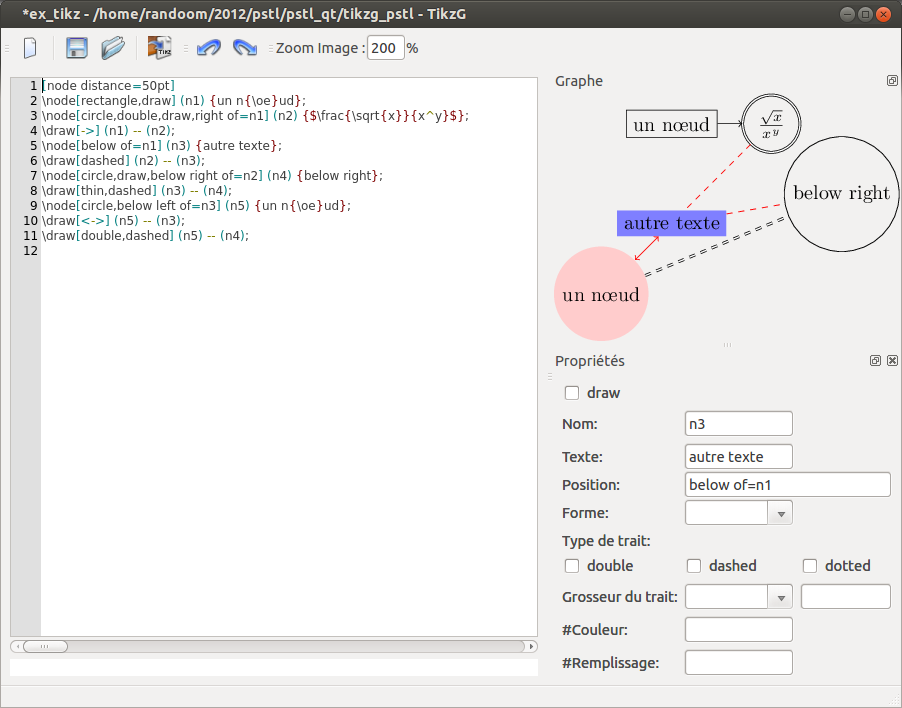
\includegraphics[width=15cm, height=10cm]{img/r_9.png}
\\ 
figures 7: modification graphique des propriétés d'un n{\oe}ud
\\
\\
Lorsqu'on clique sur un objet du graphe ses propriétés s'affichent. Prenons comme exemple les figures 7, on voit que lorsqu'on clique sur le noeud n3, il est coloré en bleu, ses noeuds relatifs en rose et les arêtes auxquelles il est rélié en rouge. A partir de sa fenêtre de propriétés on peut apporter des modifications au n{\oe}ud ainsi sélectionné. 
\section{Conclusion}
\section{Perspectives}
   

\end{document}


